\documentclass[12pt]{article}

% refer to configurations.tex for the LaTeX setup of this template
\usepackage[english]{babel}

\title{\textbf{\textsf{Tauola \\}}}
\date{\today}
\author{}

% math
\usepackage{amsmath, amssymb}

% references
\usepackage[style=apa, backend=biber]{biblatex}
\addbibresource{bibliography.bib}

% fonts
%\usepackage{helvet}
%\usepackage{sectsty}
%\allsectionsfont{\sffamily} % for section titltes use sans-serif
% \renewcommand{\familydefault}{\sfdefault} % comment out for sans-serif font
% \usepackage{sansmath} % comment out for sans-serif math font
% \sansmath % comment out for sans-serif math font

% margins
\usepackage{geometry}
\geometry{
  a4paper,
  total={170mm,257mm},
  left=25mm,
  right=25mm,
  top=30mm,
  bottom=30mm,
}

% no indentation when a new paragraph starts
\setlength{\parindent}{0cm}

% links
\usepackage{hyperref} % better links
\usepackage{color}    % nicer link colors
\definecolor{pigment}{rgb}{0.2, 0.2, 0.6}
\hypersetup{
  colorlinks = true, % Color links instead of ugly boxes
  urlcolor   = pigment, % Color for external hyperlinks
  linkcolor  = black, % Color for internal links
  citecolor  = pigment % Color for citations
}

\usepackage{graphicx}

%here is the path
\graphicspath{ {./images/} }

% headers
\usepackage{fancyhdr}
\pagestyle{fancy}
\lhead{Tauola}
\chead{}
\rhead{}

% example boxes
\usepackage{tcolorbox}
\newtcolorbox{examplebox}{
  colback=white,
  colframe=gray!30,
  title=Example,
  sharp corners,
  boxrule=0.5pt,
  coltitle=black
}

%bash script
\usepackage{minted}


% conditionals
\usepackage{ifthen}
\newboolean{showinstructions}
\newboolean{showexamples}
\newboolean{showexplanations}
\renewenvironment{examplebox}{%
  \ifthenelse{\boolean{showexamples}}%
    {\begin{tcolorbox}[colback=white, colframe=gray!30, title=Example, sharp corners, boxrule=0.5pt, coltitle=black]}%
    {\expandafter\comment}%
}{%
  \ifthenelse{\boolean{showexamples}}%
    {\end{tcolorbox}}%
    {\expandafter\endcomment}%
}

% Define a new environment for explanations
\newcommand{\explanation}[1]{%
  \ifthenelse{\boolean{showexplanations}}%
    {\textit{Explanation:} #1}%
    {\ignorespaces}%
}

% Define a new environment for instructions
\newcommand{\instructions}[1]{%
  \ifthenelse{\boolean{showinstructions}}%
    {#1}%
    {\ignorespaces}%
}

\makeatletter
\newcommand{\maketitlepage}{%
    \begin{titlepage}
        \maketitle
        \thispagestyle{empty}
        \vfill 
        \centering
        Version: 1.1.8 \\
        Last updated: 2025-03-02 \\
        Report based on the source code and papers:\\
    \url{https://tauolapp.web.cern.ch/resources/TAUOLA.1.1.8/Tauola_interface_design.1.1.8.pdf}, 
        \vfill 
    \end{titlepage}
    \newpage
}
\makeatother

% Optional user settings
\setboolean{showinstructions}{true} % set to false to hide instructions
\setboolean{showexamples}{true} % set to false to hide examples
\setboolean{showexplanations}{true} % set to false to hide explanations

\begin{document}
\maketitlepage

\section{Installation}

For Tauola installation, you need the HepMC2 and HepMC3.\\

For HepMC2 and HepMC3 package, you download the source code and create a build directory. Then run the following command from the build directory.

\begin{minted}{bash}
cmake -DCMAKE_INSTALL_PREFIX=/home/john/products/HepMC2/HepMC-2.06.11/
/home/john/products/HepMC2/HepMC-2.06.11/ -Dmomentum:STRING=GEV
-Dlength:STRING=MM
\end{minted}

For the installation of Tauola, you can do
\begin{minted}{bash}
./configure --prefix=/home/john/products/Tauola/TAUOLA
--with-hepmc=/home/john/products/HepMC2/HepMC-2.06.11/
--with-hepmc3=/home/john/products/HepMC3/HepMC3-3.3.0
--with-lhapdf=/home/john/products/LHAPDF/LHAPDF-6.5.5
--with-pythia8=/home/john/products/Pythia8/pythia8313
--with-mc-tester=/home/john/products/MC-TESTER/mc-tester
\end{minted}


\section{Tauola Subroutines}
\subsection{JAKER}
\textbf{SUBROUTINE JAKER(JAK)}\\
This subroutine selects the decay modes depending on the branching ratio. JAK is an integer that determines which tau decay mode is selected. Each JAK value corresponds to a specific decay channel (e.g., tau → electron + neutrinos).

\begin{itemize}
    \item JAK=0 - Allows according to standard model
    \item JAK=1 - electron mode ($\tau \rightarrow  e \nu_\tau \nu_e$)
    \item JAK=2 - muon mode ($\tau \rightarrow  \mu \nu_\tau \nu_\mu$)
    \item JAK=3 - pion mode ($\tau \rightarrow  \pi \nu_\tau$)
    \item JAK=4 - rho mode ($\tau \rightarrow  \rho \nu_\tau$)
    \item JAK=5 - A1 mode (axial-vector meson)($\tau \rightarrow  a1 \nu_\tau$)
    \item JAK=6 - K mode ($\tau \rightarrow  K \nu_\tau$)
    \item JAK=7 - K* mode ($\tau \rightarrow  K* \nu_\tau$)
    \item JAK=8 - n$\pi$ mode ($\tau \rightarrow  n\pi \nu_\tau$)
\end{itemize}

\subsubsection{global variables}
{\textbf{Taubra}\\
GAMPRT(30) - The partial widths (branching probabilities) of different decay modes.\\
JLIST(30) - The list of decay mode identifiers.\\
NCHAN - The number of possible decay channels.\\}

\subsubsection{local variables}
{CUMUL(30) - Stores cumulative sums of branching ratios.\\
RRR(1) - Stores a random number used for selection.\\
}\\
It ensures number of decay channels is within the valid range. If NCHAN is less than 1 or greater than 30, the program exits with an error.\\

Suppose mode 1 has 30$\%$, mode 2 has 50$\%$ and mode 3 has 20$\%$ probability, the cummuliative array will be 30, 80,100 $\%$ probabilities respectively. Then it iterate through the list of decay channel and if the random number (0,1) falles within the range, that particular decay mode is selected. The branching ratios are not filled in this subroutine\\

The decay mode identifier in JLIST is passed to JAK variable

\subsection{DEKAY}
\textbf{SUBROUTINE DEKAY(KTO,HX)}\\
This subroutine handles the decay of tau leptons, including initialization, decay mode selection, and final state transformations. \\

The IF statement and its ELSEIF branches control the program's behavior based on KTO

KTO = -1  - Initialization
KTO = 1   - $\tau^+$ decay
KTO = 2   - $\tau^-$ decay
KTO = 11  - Completing $\tau^+$ decay
KTO = 12  - Completing $\tau^-$ decay
KTO = 100 - Final Processing



\subsubsection{global variables}
\textbf{JAKI}\\
JAK1 - \\
JAK2 - \\
JAKP - \\
JAKM - \\
KTOM - \\

\textbf{IDFC}\\
IDF - \\

\textbf{TAUPOS}\\
NP1 - \\
NP2 - \\

\textbf{TAUBMC} \\
GAMPMC(30) - \\
GAMPER(30) - \\
NEVDEC(30) - \\

\textbf{TAUDCD} \\
IDFFIN(9,NMODE) -  2D array\\
MULPIK(NMODE) - \\
NAMES(NMODE)*31 - Character array\\

\textbf{INOUT}\\
INUT - \\
IOUT - \\

\subsubsection{local variables}

H(4) - temporaryily used\\
HX(4) (double) - A polarimetric vector used by the host program for calculating the spin weight of tau decay\\
GAMPMC(double) - \\
GAMPER(double) - \\
PDUM1(4),PDUM2(4),PDUM3(4),PDUM4(4),PDUM5(4) - \\
HDUM(4) - \\
PDUMX(4,9) - \\
IWARM = 0\\

\subsubsection{Constants}

NMODE=15   - Likely represents the number of decay modes available in the subroutine\\
NM1=0, NM2=1, NM3=8, NM4=2, NM5=1, NM6=3




\subsection{DADNEW}
\textbf{SUBROUTINE DADNEW(MODE,ISGN,HV,PNU,PWB,PNPI,JNPI)}\\
NMODE = 196 - Total number of decay modes handled in this subroutine.


\subsubsection{global variables}
\textbf{PARMAS}\\
This block stores masses and decay widths of fundamental particles, mainly mesons and leptons, used in the tau decay simulation.\\
AMTAU  - Mass of the $\tau$ lepton\\
AMNUTA - Mass of the $\tau_\nu$\\
AMEL   - Mass of electron\\
AMNUE  - Mass of $\nu_e$\\
AMMU   - Mass of $\mu^-$\\
AMNUMU - Mass of $\nu_\mu$\\
AMPIZ  - Mass of $\pi^0$\\
AMPI   - Mass of $\pi^-$\\
AMRO   - Mass of $\rho$ meson\\
GAMRO  - Decay width of $\rho$ meson\\
AMA1   - Mass of $A_1$ meson\\
GAMA1  - Decay width of $A_1$ meson\\
AMK    - Mass of charged Kaon\\
AMKZ   - Mass of K$^0$\\
AMKST  - Mass of K$^*$ meson\\
GAMKST - Decay width of K$^*$ meson\\


\textbf{DECPAR}\\
GFERMI - Fermi's constant $G_F$\\
GV     - Vector coupling constant for weak interactions\\
GA     - Axial-vector coupling constant\\
CCABIB - Cosine of the Cabibbo angle cos($\theta_c$), governing quark mixing in weak decays\\
SCABIB - Sine of the Cabibbo angle cos($\theta_c$), also related to quark mixing\\
GAMEL  - Partial decay width of the electron decay channel ($\tau \rightarrow e \nu_e \tau$ )\\

CCABIB and SCABIB determine decay rates involving Cabibbo-favored and Cabibbo-suppressed processes.\\

\textbf{TAUBMC}\\
GAMPMC(500)	- Stores the normalized partial decay widths for different tau decay channels\\
GAMPER(500) - Stores the uncertainty (error) in the decay widths\\
NEVDEC(500) - Stores the number of decays simulated for each channel\\

\textbf{TAUDCD}   -   Tau decay information\\
IDFFIN(9,NMODE)  - Likely represents the final-state particle IDs for each tau decay mode. 9 rows suggest that up to 9 particles can be tracked per decay mode.\\
MULPIK(NMODE) - Likely stores the multiplicity of pions ($\pi$) in each decay mode.\\
NAMES(NMODE)   - Stores the names of the decay channels.

\subsubsection{local variables}

PNU(4) - Four momentum of neutrino.\\
PWB(4) - Four vector of a particle in decay process.\\
PNPI(4,9) - Stores four-momentum components of up to 9 pions in a decay mode.\\
HV(4) - Stores a four-momentum used in computations.\\
HHV(4) - Possibly an intermediate calculation of HV(4), used for handling helicities or boosting frames.\\
PDUM1(4), PDUM2(4), PDUMI(4,9) - Dummy four-momentum variables used in calculations.\\

RRR(3) - Random number\\
WTMAX(NMODE) - Stores the maximum weight for each of the tau decay modes\\
SWT(NMODE) - Sum of weights for accepted events per decay mode.\\
SSWT(NMODE) - Sum of squared weights (used for error estimation).\\
NEVRAW(NMODE) - Total number of simulated decays per mode.\\
NEVOVR(NMODE) - Number of overweighted events per mode.\\
NEVACC(NMODE) - Number of accepted decays per mode.\\


\textbf{MODE=-1}  - triggers a specific initialization routine.\\
IWARM = 1 -  Marks the initialization as done.


What is Ntrials do? The 4$\pi$ phase space needs lot more trials at initialization (probably mentioning the number of samples),

The initialization calls different decay phase space functions (DPH4PI, DPH5PI, etc.). This is probably to establish weights. Each function likely simulates a different multi-pion decay mode. The thresholds (NM4, NM5, etc.) define how many decay modes fall into each category.\\

\vspace{0.5cm}
\textbf{MODE=0} generates the tau decays based on initialized parameters.\\
Calls decay functions (DPH4PI, DPH5PI, etc.), but now actually records events.

Rotation transformations to align with tau rest frame.\\

The $\theta$ and $\phi$ is generated randomly across a sphere. \\

The ROTOR2 subroutine rotates PNU along y-axis THET units.\\
And ROTOR3 subroutine rotates PNU along z-axis PHI units.\\

It rotates, neutrino, W-boson and Some helicity or spin-related quantity randomly and isotropically.

\vspace{0.5cm}
\textbf{MODE=1} performs statistical calculations related to decay events and prints out results.



\subsubsection{DPH1PI}
\textbf{SUBROUTINE DPH1PI(WT,HV,PNU,PWB,PNPI,JNPI)}\\

This subroutine model the decay of tau lepton($\tau$) into a neutrino and a single meson. This subroutine computes the momentum of the decay products when a tau lepton ($\tau$) decays into a neutrino and a single meson.

Following are the masses used in tau decays \\
C IN-COMING / OUT-GOING  FERMION MASSES\\
      AMTAU  = 1.7842\\
C --- let us update tau mass ...\\
      AMTAU(m$_\tau$)        = 1.777\\
      AMNUTA(m$_{\nu_\tau}$) = 0.0 $!$ 0.010   (nearly zero(0 or $\leq$0.01))\\
      AMEL(m$_{e^-}$)        = 0.0005111\\
      AMNUE(m$_{\nu_e}$)     = 0.0\\
      AMMU(m$_\mu$)          = 0.105659 \\
      AMNUMU(m$_{\nu_\mu}$)  = 0.0\\
*\\
* MASSES USED IN TAU DECAYS\\
\\
      AMPIZ(m$_{\pi_0}$)     = 0.134976\\
      AMPI(m$_\pi$)          = 0.139570\\
      AMRO(m$_\rho$)         = 0.77590\\
      GAMRO($\Gamma_\rho$)   = 0.14790\\
*C    GAMRO                  = 0.666\\
      AMA1(m$_{a1}$)         = 1.251\\
      GAMA1($\Gamma_{a1}$)   = 0.599\\
      AMK(m$_K$)             = 0.493677\\
      AMKZ(m$_{K^0}$)        = 0.497672\\
      AMKST(m$_{K^*}$)       = 0.89166\\
      GAMKST($\Gamma_{K^*}$) = 0.0508\\

Some initilization - \\

(NLT=2,NMODE=196,NM1=40,NM2=71,NM3=19,NM4=32,NM5=21,NM6=13)\\

Here INUM determines the specific decay process.

Using relativistic kinematics, the energy ($E_{KK}$,$E_\nu$) and momentum X$_{KK}$ of the meson and neutrino are given by:\\
\[E_{KK} = \frac{m_\tau^2+m_{KK}^2-m_\nu^2}{2m_\tau}\]

\[E_{\nu} = \frac{m_\tau^2-m_{KK}^2+m_\nu^2}{2m_\tau}\]

\[X_{KK} = \sqrt{E_{KK}^2-m_{KK}^2}\]

SPHERA(XKK, PKK) - Generates a random isotropic direction for the 3-momentum of the meson.\\
PKK(4) = EKK - Assigns the energy component of the meson's 4-momentum.\\
The neutrino’s 3-momentum(PNU) is the opposite of the meson's 3-momentum \\

\subsection{DAM1PI}
\textbf{SUBROUTINE DAM1PI(INUM,PNU,AMF0,PKK,AMF1,GAMM,HV)} - Line No : 3317\\

INUM - Decay channel identifier (1 for $\pi^- \nu_\tau$, 2 for $K^-\nu_\tau$)\\
PNU(4) - 4-momentum of neutrino\\
AMF0 - Mass of neutrino\\
PKK(4) - 4-momentum of the meson\\
AMF1 - Mass of the meson\\
GAMM - The decay width($\Gamma$)\\
HV(4) - \\

The decay parameters and the particle masses are loaded

The DAM1PI subroutine is responsible for computing the decay width ($\Gamma$) and angular distribution for the decay of a tau lepton ($\tau$) into a single pseudoscalar meson ($\pi$ or $K$) and a neutrino ($\nu_\tau$).\\


PXQ = AMTAU*EKK . Its just the scalar product of four momentum of tau and the meson($P_{\tau}$ $\cdot$ $P_{KK}$ = m$_\tau \cdot E_{KK}$). This is because the $\tau$ momentum is zero in $\tau$'s rest frame.\\

PXN=AMTAU*ENU. Similarly for $\nu_\tau$ also the ($P_{\tau}$ $\cdot$ $P_{\nu}$ = m$_\tau \cdot E_\nu$)\\

QXN = $P_{KK} \cdot P_\nu$ = $E_{KK}E_\nu - p_{KK} \cdot p_\nu$\\

\[BRAK = (G_V^2+G_A^2)(2P_\tau \cdot P_{KK} \cdot P_{KK} \cdot P_\nu - m_{KK}^2 P_\tau \cdot P_\nu)\ + (G_V^2 - G_A^2) m_\tau m_\nu m_{KK}^2 \]

The helicity vector HV determines the angular dependence of the decay.

\[ HV(1-3) = \frac{2G_AG_Vm_\tau (2p_{KK}(I) \cdot P_{KK} \cdot P_\nu - p_\nu(I) m_{KK}^2)}{BRAK}  \]

\[HV(4) = 1 \]

The decay width for the 2-body decay including the phase space factor.\\

INUM = 1 for $\tau^- \rightarrow \pi^- \nu_\tau$\\
INUM = 2 for $\tau^- \rightarrow K^- \nu_\tau$\\

\[\Gamma = \frac{G_F^2 f^2}{16\pi}m_\tau^3\Big(\frac{BRAK}{m_\tau^4}\Big)\sqrt{\frac{(m_\tau^2-m_{KK}^2-m_\nu^2)^2-4m_{KK}^2m_\nu^2}{m_\tau^4}}\]

f is the pion/kaon decay constant ($f_\pi$= 0.1284 and $f_{K} = 0.0354$)\\

The last part of the subroutine is made as a placeholder for the potential non-standard model modification's such as
\begin{itemize}
    \item Matrix element corrections
    \item Dalitz plot effects
    \item Other beyond-SM physics contributions
\end{itemize}

IME values\\
\begin{itemize}
    \item IME=2 decay into pion/kaon + neutrino
    \item IME=4 Another decay mode with decay constant $f$ computed externally
    \item IME=5 Calls an external wrapper (DAM1PI\_wrap), possibly for beyond-SM physics
    \item IME=0 Not initialized, assigns default values
    \item IME=Others Assumes flat phase space (basic decay model)
\end{itemize}

\subsection{DPH4PI}
\textbf{SUBROUTINE DPH4PI(DGAMT,HV,PN,PAA,PMULT,JNPI)}-Line no 3411

This subroutine simulates the decay of A1 meson in the rest frame of the $\tau$ lepton, with $A_1$ momentum aligned along the z-axis. The decay process involves generating momenta for multiple particles, handling resonances, and computing the corresponding phase-space factors.

HV(4) - Helicity vector (4-momentum of the $a_1$) \\
PT(4) - 4-momentum of the $\tau$ lepton (initialized at rest)\\
PN(4) - 4-momentum of the $\nu_\tau$\\
PAA(4) - 4-momentum of the $a_1$ meson\\
PIM1(4), PIM2(4), PIPL(4) - 4-momenta of final state charged pions\\
PIZ(4) - 4-momentum of the neutral pion\\
PR(4) - Auxiliary momentum variable used for reference frame changes\\
PMULT(4,9) - Stores momenta of multiple decay products\\ \\

UU - Likely a parameter related to kinematic calculations, such as an invariant mass squared or a phase-space variable.\\
FF, FF1, FF2, FF3, FF4 - Jacobian correction factor.\\
GG1, GG2, GG3, GG4 - Use is not clear.\\
XLAM(X,Y,Z) - Computes the Källén function $\lambda(x,y,z)$.\\

PHSPAC - $\frac{1}{2^{23}\pi^{11}}$.\\ \\
PHSP - $\frac{1}{2^5 \pi^2}$ = $\frac{1}{32 \pi^2}$.\\ \\
AMP1, AMP2, AMP3, AMP4 - Masses of the final state particles.\\
AM4SQ, AM3SQ, AM2SQ - Squared masses of 4, 3, and 2-pion systems.\\
ALP1, ALP2, ALP - Angles for resonance sampling.\\
EXE - Boost factor for Lorentz transformations.\\

CHOICE4 - Chooses resonance parameters for phase space sampling.\\

PT is initialized with the $\tau$ lepton four momentum values at rest.\\

AMP1 - $\pi^-$  mass\\
AMP2 - Another $\pi^-$  mass\\
AMP3 - $\pi^+$  mass\\
AMP4 - $\pi^0$ mass

The $\tau$ might decay to some unstable particles and they decay to other particles. The mass of a resonance is not fixed, but follows a Breit-Wigner distribution characterized by a central mass $m_\rho$ and width $ \Gamma_\rho$.


\[AMS1 = m_\pi^2 = (m_{\pi1^-} + m_{\pi2^-} + m_{\pi1^+} + m_{\pi^0})^2\]

\[AMS2 = (m_\tau - m_{\nu_\tau})^2\]


\subsubsection{4-Pion System Mass (AM4)}

\[\frac{dN}{dm_\pi} = \frac{\Gamma_\rho}{(m_\pi^2 - m_\rho^2)^2 + (m_\rho \Gamma_\rho)^2} \]


This is implemented using the inverse transform sampling method.\\

To derive the CDF for the breit-wigner distribution, we need to integrate from ${-\infty}$ to $m_\pi^2$.

\[F(m_\pi^2) = \int_{-\infty}^{m_\pi^2}  \frac{\Gamma_\rho}{(m_\pi^{'2} - m_\rho^2)^2 + (m_\rho \Gamma_\rho)^2}dm_\pi^{'2} \]

The integral has the standard form:
\[\int \frac{dx}{x^2+a^2} = \frac{1}{a}tan^{-1}\Big(\frac{x}{a}\Big)\]

where we define
\[x = m_\pi^{'2} - m_\rho^2,   \;\;\; a = m_\rho \Gamma_\rho \]

\[dx = dm_\pi^{'2}\]

This substitution transforms our integral into:

\[F(m_\pi^2) = \int_{-\infty}^{m_\pi^2-m_\rho^2}  \frac{\Gamma_\rho}{x^2 + (m_\rho \Gamma_\rho)^2}dx\]
%\frac{dx}{2\sqrt{x+m_\rho^2}} \]

Applying the standard integral formula:

\[F(m_\pi^2) = \frac{1}{m_\rho \Gamma_\rho} \Bigg[ \frac{\pi}{2} + tan^{-1}\Big( \frac{m_\pi^2-m_\rho^2}{m_\rho \Gamma_\rho}\Big) \Bigg]\]

Now we have to invert the CDF for sampling,

\[F(m_\pi^2) = U\]

where U is the uniform random number form [0,1] and solve for $m_\pi^2$

\[Um_\rho \Gamma_\rho - \frac{\pi}{2} = tan^{-1}\Bigg( \frac{m_\pi^2-m_\rho^2}{m_\rho \Gamma_\rho} \Bigg)\]

\[tan (Um_\rho \Gamma_\rho - \frac{\pi}{2}) = \frac{m_\pi^2-m_\rho^2}{m_\rho \Gamma_\rho}\]

Solving for $m_\pi^2$,
\[m_\pi^2 =  m_\rho^2 + m_\rho \Gamma_\rho tan(Um_\rho \Gamma_\rho - \frac{\pi}{2})\]


From the code its,

\[ ALP1 = tan^{-1}\Big(\frac{m_\pi^2- m_\rho^2}{m\rho \Gamma_\rho}\Big)\]


\[ALP2 = tan^{-1}\Big(\frac{(m_\tau - m_{\nu_\tau})^2- m_\rho^2}{m\rho \Gamma_\rho}\Big)\]

\[ALP = ALP1+ U(ALP2-ALP1)\]

\[m_\pi^2 =  m_\rho^2 + m_\rho \Gamma_\rho tan(ALP)\]

Has to see how the difference arise........................\\

\vspace{1cm}

THREE BODY PHASE SPACE NORMALIZED AS IN BJORKEN-DRELL\\

The phase space weight PHSPAC is updated based on this resonance shape.

\[PHSPAC = \frac{1}{2^{23}\pi^{11}}\Big( \frac{(m_\pi^2-m_\rho^2)^2+ (m\rho \Gamma_\rho)^2}{m_\rho \Gamma_\rho}\Big) \times (ALP2-ALP1)\]


%\\The jacobian mentioned in the code refers to the Jacobian factor used to adjust for the phase space volume element in a Monte Carlo simulation of particle decays. The Jacobian is essential when transforming from one set of variables (e.g., the initial particle momenta or energies) to another (e.g., the momenta or energies of the decay products in the final state).

\subsubsection{3-Pion System Mass (AM3)}

The program determines whether to use a flat phase space sampling or include another resonance (like $\omega$). $\omega$ is sampled in the three pion system with a narrower Breit-Wigner shape. \\

If a second random number RRR(9) is greater than a threshold (PREZ), a flat phase space model is used:

\[m_{3\pi}^2 = ( m_{\pi2^-} + m_{\pi1^+} + m_{\pi^0})^2 + U* \Big((m_\pi - m_{\pi1^-})^2 - ( m_{\pi2^-} + m_{\pi1^+} + m_{\pi^0})^2\Big)\]


Note that one pion is less\\

Otherwise, a Breit-Wigner sampling for the omega meson ($\omega$) is applied, using a method similar to the $\rho$ resonance treatment above.\\

Jacobian factor FF1, if its flat phase space is

\[FF1 = (m_\pi - m_{\pi1^-})^2 - ( m_{\pi2^-} + m_{\pi1^+} + m_{\pi^0})^2\]

If its Breit-Wigner,

\[FF1 = \frac{(m_{3\pi}^2 -m_\omega^2)^2 + (m_\omega \Gamma_\omega)^2}{m_\omega \Gamma_\omega} \times (ALP2-ALP1)\]

\subsubsection{2-Pion System Mass (AM2)}

A similar method is applied for the two-pion invariant mass.\\
It uses flat phase space sampling.

The Jacobian term for this is stored in FF2

\subsubsection{Final 2-Pion Kinematics in the Rest Frame}
The program computes the energies of two final-state pions in the rest frame:

\[E_{\pi^0} = \frac{m_{2\pi}^2- m_{\pi^+}^2+m_{\pi^0}^2}{2m_{2\pi}}\]
\[E_{\pi^+} = \frac{m_{2\pi}^2+ m_{\pi^+}^2-m_{\pi^0}^2}{2m_{2\pi}}\]
\[p_{\pi^0} = \sqrt{E_{\pi^0}^2 - m_{\pi^0}^2}\]

\[PHSPAC = PHSPAC \times 4\pi \times (\frac{2 p_{\pi^0}}{m_{2\pi}}) \]








PR is the momentum of the intermediate particle (2pi system). \\

\[PR(1) = 0\]
\[PR(2) = 0\]
\[PR(4) = E_{PR} = \frac{m_{3\pi}^2+m_{2\pi}^2- m_{\pi^-}^2}{2m_{3\pi}}\]
\[PR(3) = \sqrt{abs(E_{PR}^2-m_{2\pi}^2)} \]

PIM1 - momentum of the $\pi^-$

\[PIM1(1) = 0\]
\[PIM1(2) = 0\]
\[PIM1(4) = E_{\pi^-} = \frac{m_{3\pi}^2-m_{2\pi}^2+ m_{\pi^-}^2}{2m_{3\pi}}\]
\[PIM1(3) = -PR(3)\]

This following factor accounts for the Jacobian when transforming between momentum variables.
\[FF3 = 4\pi\frac{2 p_{z,2\pi}}{m_{3\pi}}\]


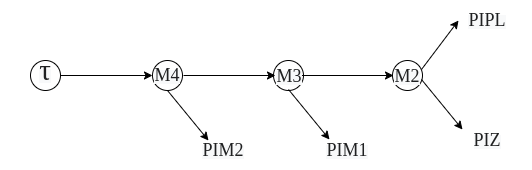
\includegraphics[width=14cm]{tauola_4pion.drawio.png}

\subsubsection{Boosting}

The BOSTER3(EXE,PVEC,QVEC) subroutine boost PVEC with EXE and outputs the boosted one in QVEC.

Here \[EXE = e^\eta, \;\;\;\;\; where \;\;\; \eta \;\; is \;\;  the \;\; hyperbolic \;\; velocity\]

\[e^\eta = cosh \eta + sinh \eta = \frac{E}{M}+\frac{p_z}{M}\]


\[EXE= e^\eta  = \frac{PR(4) +PR(3)}{m_{2\pi}}\]


Coming to the Boost subroutine

\[QVEC(4) = E^{'} =  \frac{(E+p_z)e^\eta + (E-p_z)e^{-\eta}}{2}\]

\[QVEC(3) = p_z^{'} =  \frac{(E+p_z)e^\eta - (E-p_z)e^{-\eta}}{2}\]


We do the boosting to PIZ and PIPL to $m_{2\pi}$'s frame. Then we apply random rotation to PIPL, PIM1, PIZ and $m_{2\pi}$.\\

Then we will solve for the four vector of $m_{3\pi}$ and PIM2. \\

Later we will again boost PIZ, PIPL, PIM1 to $m_{3\pi}$'s frame. Then we will apply random rotation to PIPL, PIM1, PIM2, PIZ and $m_{3\pi}$\\

The last step is finding $m_{4\pi}$ four momentum(PAA) and the neutrino four momentum(PN).\\

There is no boosting done on this. \\

There is a swapping of PIM1 and PIM2 momentum for a small fraction of events. The reason is
not clear to me at this time. It's mentioned in the code as a bug fix.


The jacobian factors calculated earlier are not used. They are recalculated in the following sections.

\subsubsection{Flat Phase Space Channel}
Recalculate the $m_{3\pi}$ from the calculated momentum of the three pions.

\[m_{3\pi}^2 = AM3SQ \]
\[= (E_{\pi^-}+E_{\pi^+}+E_{\pi^0})^2 - (pz_{\pi^-}+pz_{\pi^+}+pz_{\pi^0})^2- (py_{\pi^-}+py_{\pi^+}+py_{\pi^0})^2- (px_{\pi^-}+px_{\pi^+}+px_{\pi^0})^2\]

\[AMS1 = (m_{\pi2^-} + m_{\pi^+} + m_{\pi^0})^2\]
\[AMS2 = (m_{4\pi}-m_{\pi^-})^2\]

\[FF1 = AMS2 - AMS1\]

\[AMS1 = (m_{\pi1^+} + m_{\pi^0})^2\]
\[AMS2 = (m_{3\pi}-m_{\pi2^-})^2\]


\[FF2=AMS2-AMS1\]

\[FF3 =  4\pi \frac{\lambda^{1/2}(m_{3\pi}^2, m_{2\pi}^2, m_{\pi2^-}^2)}{m_{3\pi}^2}\]

\[FF4 =  4\pi \frac{\lambda^{1/2}(m_{4\pi}^2, m_{3\pi}^2, m_{\pi1^-}^2)}{m_{4\pi}^2}\]

\[UU = FF1 \times FF2 \times FF3 \times FF4\]

\[UU = \Big((m_{4\pi}-m_{\pi^-})^2 - (m_{\pi2^-} + m_{\pi1^+} + m_{\pi^0})^2\Big) \times
	\Big( (m_{3\pi}-m_{\pi^-})^2 - (m_{\pi^+} + m_{\pi^0})^2\Big)  \]
	\[\times 4\pi \frac{\lambda^{1/2}(m_{3\pi}^2, m_{2\pi}^2, m_{\pi^-}^2)}{m_{3\pi}^2} \times
	4\pi \frac{\lambda^{1/2}(m_{4\pi}^2, m_{3\pi}^2, m_{\pi^-}^2)}{m_{4\pi}^2} \]


\subsubsection{Breit Wigner Phase Space Channel}

\[m_{3\pi}^2 = AM3SQ \]
\[= (E_{\pi^-}+E_{\pi^+}+E_{\pi^0})^2 - (pz_{\pi^-}+pz_{\pi^+}+pz_{\pi^0})^2- (py_{\pi^-}+py_{\pi^+}+py_{\pi^0})^2- (px_{\pi^-}+px_{\pi^+}+px_{\pi^0})^2\]

\[AMS1 = (m_{\pi2^-} + m_{\pi^+} + m_{\pi^0})^2\]
\[AMS2 = (m_{4\pi}-m_{\pi^-})^2\]

\[ALP1 = tan^{-1}\Big(\frac{(m_{\pi2^-} + m_{\pi^+} + m_{\pi^0})^2 - m_\rho^2}{m_\rho \Gamma_\rho}\Big)\]

\[ALP2 = tan^{-1}\Big(\frac{(m_{4\pi}-m_{\pi^-})^2 - m_\rho^2}{m_\rho \Gamma_\rho}\Big)\]


\[FF1 = \frac{(m_{3\pi}^2 - m_\rho^2)^2 + 	m_\rho^2 \Gamma_\rho^2}{m_\rho \Gamma_\rho} \times \Bigg(tan^{-1}\Big(\frac{(m_{4\pi}-m_{\pi^-})^2 - m_\rho^2}{m_\rho \Gamma_\rho}\Big) -  tan^{-1}\Big(\frac{(m_{\pi2^-} + m_{\pi^+} + m_{\pi^0})^2 - m_\rho^2}{m_\rho \Gamma_\rho}\Big)  \Bigg)\]


\[AMS1 = (m_{\pi1^+} + m_{\pi^0})^2\]
\[AMS2 = (m_{3\pi}-m_{\pi2^-})^2\]


\[FF2=AMS2-AMS1\]

\[FF3 =  4\pi \frac{\lambda^{1/2}(m_{3\pi}^2, m_{2\pi}^2, m_{\pi2^-}^2)}{m_{3\pi}^2}\]

\[FF4 =  4\pi \frac{\lambda^{1/2}(m_{4\pi}^2, m_{3\pi}^2, m_{\pi1^-}^2)}{m_{4\pi}^2}\]


\[FF = FF1 \times FF2 \times FF3 \times FF4\]


\subsubsection{Second Channel With Breit Wigner}

\[m_{3\pi}^2 = AM3SQ \]
\[= (E_{\pi2^{-}}+E_{\pi^+}+E_{\pi^0})^2 - (pz_{\pi2^{-}}+pz_{\pi^+}+pz_{\pi^0})^2- (py_{\pi2^-}+py_{\pi^+}+py_{\pi^0})^2- (px_{\pi2^-}+px_{\pi^+}+px_{\pi^0})^2\]

\[AMS1 = (m_{\pi1^-} + m_{\pi^+} + m_{\pi^0})^2\]
\[AMS2 = (m_{4\pi}-m_{\pi2^-})^2\]

\[ALP1 = tan^{-1}\Big(\frac{(m_{\pi1^-} + m_{\pi^+} + m_{\pi^0})^2 - m_\rho^2}{m_\rho \Gamma_\rho}\Big)\]

\[ALP2 = tan^{-1}\Big(\frac{(m_{4\pi}-m_{\pi2^-})^2 - m_\rho^2}{m_\rho \Gamma_\rho}\Big)\]


\[GG1 = \frac{(m_{3\pi}^2 - m_\rho^2)^2 + 	m_\rho^2 \Gamma_\rho^2}{m_\rho \Gamma_\rho} \times \Bigg(tan^{-1}\Big(\frac{(m_{4\pi}-m_{\pi2^-})^2 - m_\rho^2}{m_\rho \Gamma_\rho}\Big) -  tan^{-1}\Big(\frac{(m_{\pi1^-} + m_{\pi^+} + m_{\pi^0})^2 - m_\rho^2}{m_\rho \Gamma_\rho}\Big)  \Bigg)\]


\[AMS1 = (m_{\pi1^+} + m_{\pi^0})^2\]
\[AMS2 = (m_{3\pi}-m_{\pi1^-})^2\]


\[GG2=AMS2-AMS1\]

\[GG3 =  4\pi \frac{\lambda^{1/2}(m_{3\pi}^2, m_{2\pi}^2, m_{\pi1^-}^2)}{m_{3\pi}^2}\]

\[GG4 =  4\pi \frac{\lambda^{1/2}(m_{4\pi}^2, m_{3\pi}^2, m_{\pi2^-}^2)}{m_{4\pi}^2}\]


\[GG = GG1 \times GG2 \times GG3 \times GG4\]


Here ALP1 and ALP2 are from the initial calculations

\[PHSPAC = \frac{1}{2^{23}\pi^{11}}\Big( \frac{(m_\pi^2-m_\rho^2)^2+ (m\rho \Gamma_\rho)^2}{m_\rho \Gamma_\rho}\Big) \times (ALP2-ALP1) \times 4\pi \times (\frac{2 p_{\pi^0}}{m_{2\pi}}) \times 4\pi \frac{2p_{4\pi}}{m_\tau}\]


Not going into matrix element calculations.

\newpage
{\color{blue}
\section{5-body phase space of TAUOLA}
\begin{align}
    ENQ1 = E_{4} &= \frac{M_{2}^2- m_{3}^2+m_{4}^2}{2M_{2}} \\
ENQ2=E_{3} &= \frac{M_{2}^2+ m_{3}^2-m_{4}^2}{2M_{2}} \\
PPPI= |\mathbf{p_{4}}| &= |\sqrt{E_{4}^2 - m_{4}^2}| \\
PHSPAC &= PHSPAC \times 4\pi \times (\frac{2 p_{4}}{M_{2}})
\end{align}
Limit on $M_2^2$, $M_4$ is sourced from $\rho$-resonance (need one random number generator $\text{RR1}$).
\begin{align}
    M_{3_{\text{max}}}^2 &= (M_4 - m_1)^2 \\
     M_{3_{\text{min}}}^2 &= (m_2 + m_3 + m_4)^2
      \\
     M_3^2 &=  M_{3_{\text{min}}}^2 + RR1 * ( M_{3_{\text{max}}}^2 -  M_{3_{\text{min}}}^2) \\
    M_{2_{\text{max}}}^2 &= (M_3 - m_2)^2 \\
    M_{2_{\text{min}}}^2 &= (m_3 + m_4)^2 \\
    M_2^2 &= (m_3+m_4)^2 + RR2 * (M_3 - m_2)^2
\end{align}


The SPHERA subroutine generates a random 3D vector uniformly distributed on a sphere of radius $p_{\pi^0}$ and returns to variable PIZ.\\
 PIZ :  Four momentum of $m_4$, SPHERA (PPPI,PIZ) returns 3 vector $\mathbf{p_{\pi^0}}$\\
$PIZ = p_{4} = (E_{4}, \, p_{4} \sin{\theta} \cos{\phi}, \, p_{4} \sin{\theta} \sin{\phi}, \,  p_{4} \cos{\theta} )$\\
From momentum conservation in the rest frame,
\begin{align}
   \mathbf{p_3} &= -\mathbf{p_4} \,, \\
  PIPL =  p_{3} &=  (E_{3}, \,- p_{4} \sin{\theta} \cos{\phi}, \, -p_{4} \sin{\theta} \sin{\phi}, \, - p_{4} \cos{\theta}  ) \,\\
  PIZ = p_{4} &= (E_{4}, \, p_{4} \sin{\theta} \cos{\phi}, \, p_{4} \sin{\theta} \sin{\phi}, \,  p_{4} \cos{\theta} )
\end{align}

%%%%%%%%%%%%%%%%%%%%%%%%%%%%%%%%%%%%%%%%%%%%%%%%%%%%%%%%%%%%%%%%%%%%%%%%%%%%%%%%%

\subsubsection{Finding the 4-momentum of the intermediate particle}
{\color{blue}
\begin{align}
    E_2 &= \frac{M_3^2 - M_2^2 + m_2^2}{2M_3} \\
    E_{M_2} &= \frac{M_3^2 + M_2^2 - m_2^2}{2M_3} \\
    p_{M_{2_z}} &= |\sqrt{E_{M_2}^2 - M_2^2} |\\
     p_{2_z} &= -  p_{M_{2_z}} \\
     FF3 &= 4 \pi \frac{2 p_{M_{2_z}}}{M_3}
\end{align}
\textbf{Quick Notes on Boosted Frame:}

Let us consider two inertial frames, $F$ and $F^\prime$, where we consider $F^\prime$ has a relative velocity $v$ with respect to $F$ along the $z$-direction. All the \textit{prime} co-ordinates refer to $F^\prime$ frame. Then by using the Lorentz transformation the relation between the energy-momentum between these two frame are as follows,
\begin{align}
    \gamma &= \frac{1}{\sqrt{1+\beta^2}} \,,\\
    E^\prime &= \gamma (E + \beta p_z) \,, \\
    p^\prime _z &= \gamma (p_z + \beta E)\,, \\
    p^\prime_x &=  p_x \,,~~~~~~~~~ p^\prime_y = p_y \,.
\end{align}
Now, let us define,
\begin{align}
    \cosh{\eta} &= \gamma \,, ~~~~ \sinh{\eta} = \gamma \beta \,,\\
    \tanh{\eta} &= \beta \,. ~~~~ \eta = \tanh^{-1}{\beta} \,.\\
    \cosh{\eta} + \sinh{\eta} &= \exp{\eta} \,.
\end{align}
Therefore, using this new notation, we can define the relation between the two frames of reference as,
\begin{align}
\label{Eq:boosted_energy}
    E^\prime &= \cosh{\eta} E + \sinh{\eta} p_z \, \\
             &= \frac{e^\eta}{2} (E + p_z) + \frac{e^{-\eta}}{2} (E - p_z) \nonumber \\
    p^\prime &= \sinh{\eta} E + \cosh{\eta} p_z \,, \\
    \label{Eq:boosted_momentum}
             &= \frac{e^\eta}{2} (E + p_z) - \frac{e^{-\eta}}{2} (E - p_z)
\end{align}
Now if a particle of mass $M$ is in rest in the frame $F$ then,
\begin{align}
    E^\prime_M &= \gamma M \, ~~~~~~  p_{z_M} = \gamma \beta M \,
\end{align}
Then by using Eq. \ref{Eq:boosted_energy} and \ref{Eq:boosted_momentum} we have
\begin{align}
    \cosh{\eta} &= \gamma = \frac{E^\prime_M}{M} \,, ~~~~~~~~ \sinh{\eta}   = \gamma \beta = \frac{p_{z_M}}{M} \,,\\
    e^\eta &= \frac{E^\prime_M + p_{z_M}^\prime}{M}
\end{align}
\textbf{ BOSTR3 subroutine:} The BOSTER3(EXE,PVEC,QVEC) subroutine boost PVEC with EXE and outputs the boosted one in QVEC.

Here \[EXE = e^\eta, \;\;\;\;\; where \;\;\; \eta \;\; is \;\;  the \;\; hyperbolic \;\; velocity\]

Coming to the Boost subroutine
\[PVEC(4) = E \,, ~~~~~~ PVEC(3) = p_z\]

\[QVEC(4) = E^{'} =  \frac{(E+p_z)e^\eta + (E-p_z)e^{-\eta}}{2}\]

\[QVEC(3) = p_z^{'} =  \frac{(E+p_z)e^\eta - (E-p_z)e^{-\eta}}{2}\]
---------------------------------------------------------------------------------------------------------------------
%%%%%%%%%%%%%%%%%%%%%%%%%%%%%%%%%%%%%%%%%%%%%%%%%%%%%%%%%%%%%%%%%%%%%%%%%%%%%%%%%%%%%%%%%%%%%%%%%%%%%%%%%%%%%%%%%%%
Now, we need to boost the momentum of $m_3$ and $m_4$ in the boosted from of $M_2$. Thus from the previous understanding, we can see,
\begin{align}
    EXE= e^\eta &=\frac{p_{M_{2_z}} + E_{M_{2_z}}}{M_2} \,,\\
    E_3^\prime &= \frac{(E_3 + p_{3_z}) e^\eta + (E_3 - p_{3_z})e^{-\eta}}{2} \,,\\
    p_{3_z}^\prime &= \frac{(E_3 + p_{3_z}) e^\eta - (E_3 - p_{3_z})e^{-\eta}}{2} \,, \\
    p_{3_x}^\prime &= p_{3_x} \,, ~~~~~~~ p_{3_y}^\prime = p_{3_y} \\
    %
    E_4^\prime &= \frac{(E_4 + p_{4_z}) e^\eta + (E_4 - p_{4_z})e^{-\eta}}{2} \,,\\
    p_{4_z}^\prime &= \frac{(E_4 + p_{4_z}) e^\eta - (E_4 - p_{4_z})e^{-\eta}}{2} \,, \\
    p_{4_x}^\prime &= p_{4_x} \,, ~~~~~~~ p_{4_y}^\prime = p_{4_y}
\end{align}
Thus all the 4-vectors can be written as,
\begin{align}
\label{Eq:m_3_rest_frame}
    p_{M_2} &=(E_{M_2}, 0 , 0 ,|\sqrt{E_{M_2}^2 - M_2^2}|) \,,\\
    p_{2} & = (E_2, 0, 0, - |\sqrt{E_{M_2}^2 - M_2^2}|) \,, \\
    p_3^\prime & = (E_3^\prime, p_{3_x},  p_{3_y} , p_{3_z}^\prime) \,,\\
    p_3^\prime & = (E_4^\prime,  p_{4_x}^prime,  p_{4_y}^\prime, p_{4_z}^\prime)
\end{align}

Now, here we assume the boost of $M_2$ along the $z-$ axis which we are not sure about. So, we need to rotate the vectors in an arbitrary direction. To do so we call the $\text{ROTPOL}$ subroutine.

\textbf{ROTPOL(THET, PHI,PP) Subroutine:}

PP: is four vector

THET: Angle of rotation between $z-x$ axis
PHI: Angle of rotation between $x-y$ axis
For rotation the code use $\text{ROTOR1,2,3}$ to rotate between $y-z$, $x-z$ and $x-y$ axis. In ROTPOL $\text{ROTOR 2,3}$ are used consecutively.

Let us now check how it affects a vector which was previously in $z$ direction,

By application of ROTOR2,
\begin{align}
    p_x^\prime &= \sin{\theta} p_z, ~~~~ p_y^\prime = p_y = 0, ~~~~ p_z^\prime = \cos{\theta}p_z, ~~~~ E^\prime = E
\end{align}
By application of ROTOR3,
\begin{align}
\label{Eq:rot_z}
    p_x^{*} &= p_z \cos{\phi}\sin{\theta} , ~~~~ p_y^{*} = p_z \sin{\phi}\sin{\theta}, ~~~~ p_z^{*} = p_z \cos{\theta}, ~~~~ ~~~~ E^{\prime \prime} = E
\end{align}

Let us now check how it affects a vector which was previously in arbitrary direction,

By application of ROTOR2,
\begin{align}
    p_x^\prime &= p_x \cos{\theta} + p_z \sin{\theta} , ~~~~ p_y^\prime = p_y, ~~~~ p_z^\prime = -p_x \sin{\theta} + \cos{\theta}p_z, ~~~~ E^\prime = E
\end{align}
By application of ROTOR3,
\begin{align}
\label{Eq:rot_gen}
    p_x^{*} &= p_x^\prime \cos{\phi} - p_y^\prime \sin{\phi}  , ~~~~ p_y^{*} = p_x^\prime \sin{\phi} + p_y^\prime \cos{\phi}  ~~~~ p_z^{*} = -p_x \sin{\theta} + p_z \cos{\theta} ~~~~ E^{\prime \prime} = E
\end{align}
-----------------------------------------------------------------------------------------------------

Thus by using the ROTPOL subroutine we rotate all the vectors given in Eq.\ref{Eq:m_3_rest_frame} accordingly. $p_{M_2}$ and $p_2$ will follow eq.\ref{Eq:rot_z} and $p_{3,4}^\prime$ will follow Eq. \ref{Eq:rot_gen}.

Now we shall move to the rest frame of $M_4$, where we shall follow the same steps.
\begin{align}
    E_{M_3} &= \frac{M_4^3 + M_3^2 - m_1^2 }{2M_4}\,,\\
    p_{M_{3_z}} &= \sqrt{| E_{M_3}^2 - M_3^2|} \,,\\
    E_1 &= \frac{M_4^3 - M_3^2 + m_1^2 }{2M_4}\,,\\
    p_{m_{1_z}} &= -p_{M_{3_z}}
\end{align}
Now, the first work is to boost the momentum of the $2,3$ and $4$. No need to consider the momentum of $M_2$ now. Thus, by using the BOSTR3 (EXE, PVEC,QVEC) we boost the momentum $p_{2}^*, p_{3}^{\prime,*}, p_4^{\prime,*}$ \footnote{$*$ denotes one operation of Rotation and $\prime$ denotes the one operation boost}.
In this scenario the boost factor would be  $EXE = \frac{E_{M_3} + p_{M_{3_z}}}{M_3}$. Thus after boost the momentum becomes $p_2^{*,\prime}, p_{3}^{\prime,*,\prime}, p_4^{\prime,*,\prime}$
 Now in the similar way we also perform the rotation, and call the rotation subroutine ROTPOL and we get  $p_1^*,p_2^{*,\prime,*}, p_{3}^{\prime,*,\prime,*}, p_4^{\prime,*,\prime,*}, p_{M_3}^*$.

------------------------------------------------------------------------------------

 Now next step is to go to Tau rest frame. Here we define,
 \begin{align}
     E_{M_4} &= \frac{M_\tau^2 - m_{\nu_\tau}^2 + M_4^2}{2 m_\tau} \,, \\
     p_{M_{4_z}} &= \sqrt{|E_{M_4}^2 - M_4^2|} \,, \\
     p_{\nu_z} &= - p_{M_{4_z}} \,,
    \\
     E_{\nu_\tau} &=  \frac{M_\tau^2 + m_{\nu_\tau}^2 - M_4^2}{2 m_\tau}
 \end{align}
\begin{align}
    M_3^2 = (E_2 + E_3 + E_4)^2 - (p_{2_x}^{2} +  p_{3_x}^{2} + p_{4_x}^{2})^2 -  (p_{2_y}^{2} +  p_{3_y}^{2} + p_{4_y}^{2})^2 - (p_{2_z}^{2} +  p_{3_z}^{2} + p_{4_z}^{2})^2 \,,
\end{align}
Here the momentum are the rotated final momentum that we have derived earlier that is, $p_2^{*,\prime,*}, p_{3}^{\prime,*,\prime,*}, p_4^{\prime,*,\prime,*}$.
Now, let us define the weight factor for the integration of $M_3$,
\begin{align}
    M_{3_\text{min}}^2 &= (m_3+m_2+m_4)^2 \,, ~~~~ M_{3_{\text{max}}}^2 = ( M_4^2 - m_1^2)^2 \,,\\
    FF1 &= M_{3_{\text{max}}}^2 -  M_{3_\text{min}}^2 \,, \\
    \text{Reason:} \,\,\, M_3^2 &=  M_{3_{\text{min}}}^2 + RR1 * \underline{( M_{3_{\text{max}}}^2 -  M_{3_{\text{min}}}^2)} \,,
\end{align}
Now we need weight factor for $M_2$, \\
\begin{align}
    M_{2_{\text{min}}} &= (m_3 + m_4)^2 \\
    M_{2_{\text{max}}} & = (M_3^2 - m_1^2)
    FF2 = M_{2_{\text{max}}} -  M_{2_{\text{min}}}
\end{align}
Now, we need to add the phase space factor for the full calculation, those are,
\begin{align}
    FF3 &= 4 \pi \frac{x\lambda(M_3^2, M_2^2, m_2^2)}{M_3^2} \,,\\
    FF4 &= 4 \pi \frac{x\lambda(M_4^2, M_3^2, m_1^2)}{M_4^2} \,, \\
    FF5_{the} &= 4 \pi \frac{x\lambda(M_2^2, m_3^2, m_4^2)}{M_2^2} = 4 \pi \frac{2 p_3}{M_2} \,,\\
    UU &= FF1 * FF2 * FF3 *FF4
\end{align}
  Now in the code, $PHSPAC = \frac{1}{2^{23} \pi^{11}} (4 \pi) (2 \frac{p_1}{m_\tau}) (4 \pi) (2 \frac{p_3}{M_2}) *UU $
  \begin{align}
      PHSPAC &= \frac{1}{2^{23} \pi^{11}} (4 \pi)  \frac{x\lambda(M_2^2, m_3^2, m_4^2)}{M_2^2} (4 \pi) \frac{x\lambda(M_3^2, M_2^2, m_2^2)}{M_3^2} \nonumber \\
      &(4 \pi) \frac{x\lambda(M_4^2, M_3^2, m_1^2)}{M_4^2} (4 \pi) \frac{x\lambda(m_\tau^2, m_{\nu_\tau}^2, M_4^2)}{m_\tau^2}
  \end{align}
  So, this is 5-body phase space. Now the only parameter whose value we do not know is $M_4$- four pion mass system. Now, for this we move to the resonance scenario.

\textbf{Notes on Breit Weigner Scenario:}

  Now for a resonance channel with mass $M^*$, the matrix element is refined the the Narrow-width approximation, the propagator is,
  \begin{align}
      G^2 &= \frac{1}{(s - M^{*^2})^2 - (\Gamma^* M^*)^2}, \text{where } \Gamma^* \text{ is the decay width of $M^*$}
  \end{align}
  Now, for many body final state the resonance may appear between any collection of particles. Now, for instance let us assume the resonance in between particle $2-3$, therefore, during the break down of many particle phase space into two body phase space this will appear

  \begin{align}
     BWF &=  \int_{(m_2 + m_3)^2}^{(M-m_1)^2}{dM_{23}^2 \frac{1}{(M_{23}^2 - M^{*{2}})^2 - (\Gamma^* M^*)^2}} \, \\
     &=  \int_{(m_2 + m_3)^2 - M^{*^2}}^{(M-m_1)^2 - M^{*^2}}{d \tilde{M_{23}}^2 \frac{1}{(\tilde{M_{23}}^2)^2 - (\Gamma^* M^*)^2}} , \,, \text{where, } \tilde{M_{23}} = (M_{23}^2 - M^{*{2}}) \\
     &= \frac{1}{\Gamma^* M^*} \left( \tan^{-1}\left(\frac{(M-m_1)^2 - M^{*^2}}{\Gamma^* M^*}\right) - \tan^{-1}\left( \frac{(m_2 + m_3)^2 - M^{*^2}}{\Gamma^* M^*} \right)\right)
  \end{align}
 ---------------------------------------------------------------------------------------

 Now, let us focus on the pion system of the code, first we shall discuss about the $\rho$-resonance which happens for 4 pion system that is it depends on the mass $M_4$.
 Therefore, comparing it with the $BWF$ calculation,
 \begin{align}
     M &= m_\tau \,, ~~~~ m_1 = m_{\nu_\tau}\,, ~~~~ m_2 + m_3 = m_1+m_2+m_3+m_4 \,,\\
     M^* &= m_{\rho} \,, ~~~~ \Gamma^* = \Gamma_{\rho}
 \end{align}
 Now, in the code,
 \begin{align}
     ALP2 &= \tan^{-1}\left(\frac{(M-m_{\nu_\tau})^2 - m_\rho^2}{\Gamma_\rho m_\rho}\right) \,, ~~~~ ALP1 = \tan^{-1}\left( \frac{(m_1 + m_2 + m_3 +m_4)^2 - M^2_\rho}{\Gamma_\rho m_\rho} \right) \,,\\
     ALP &= ALP1 + R* (ALP2 - ALP1) \,,\\
     &= \tan^{-1}\left(\frac{M_4^2 - M_\rho^2}{\Gamma_\rho m_\rho}\right) \,,\\
     M_4^2 &= m_\rho^2 + \Gamma_\rho m_\rho \tan{(ALP)} \,. \\
     dM_4^2 &= \Gamma_\rho m_\rho \sec^2{ALP} \, d(ALP) \nonumber \\
     &=  \Gamma_\rho m_\rho (1+ \tan^2{ALP}) \, d(ALP) \nonumber \\
     &=  \Gamma_\rho m_\rho \left(1+ \left(\frac{M_4^2 -m_\rho^2}{\Gamma_\rho m_\rho} \right)^2 \right) \, d(ALP) \nonumber\\
     &= \frac{1}{\Gamma_\rho m_\rho} \left( \Gamma_\rho^2 m_\rho^2 + (M_4^2 - m_\rho^2)^2\right)\,  d(ALP) \,,\\
     &= \frac{1}{\Gamma_\rho m_\rho} \left( \Gamma_\rho^2 m_\rho^2 + (M_4^2 - m_\rho^2)^2\right) \times (ALP2 -ALP1) \, d(R) \,.
 \end{align}
Therefore, the phase space factor,
\begin{align}
    PHSPAC = \frac{1}{2^{23} \pi^{11}} \frac{1}{\Gamma_\rho m_\rho} \left( \Gamma_\rho^2 m_\rho^2 + (M_4^2 - m_\rho^2)^2\right) \times (ALP2 -ALP1)
\end{align}
Now, let us go for $\omega$ -resonance.
\begin{align}
    M_3 &= (m_1+m_2+m_3)^2 + R*(M_4 - m_1)^2 \,. \\
    ALP2 &= \tan^{-1}\left(\frac{(M_4-m_{1})^2 - m_\omega^2}{\Gamma_\omega m_\omega}\right) \,, ~~~~ ALP1 = \tan^{-1}\left( \frac{( m_2 + m_3 +m_4)^2 - m^2_\omega}{\Gamma_\omega m_\omega} \right) \,,\\
     ALP &= ALP1 + R* (ALP2 - ALP1)
\end{align}
  Then following the same steps, weight factor arising duet o change of variable in this case will be,
  \begin{align}
    FF1 &=   \frac{1}{\Gamma_\omega m_\omega} \left( \Gamma_\omega^2 m_\omega^2 + (M_4^2 - m_\omega^2)^2\right) \times (ALP2 -ALP1)
  \end{align}
  Now, for calculation, we go for $M_3$ defined earlier in Eq.\ref{},







  }
\newpage
\section{Doubts}
\begin{enumerate}
    \item line 3503 $AM2SQ$ is defined, then in 3533 why $AM2**2$ is used?
    \item 3514 prefactor $PHSPAC$ is not understood.
    \item 3543 phase space factor
    \item BOSTR3 (REAL) and BOSTD3 (DOUBLE PRECISION) factor are only differ by precision ????
\end{enumerate}
\newpage
\section*{References}
\nocite{Siepe2024}
\printbibliography[heading=none]

\end{document}